

\section{Appendix}




\subsection{Applications and Experiments}

\begin{figure*}
    \centering
    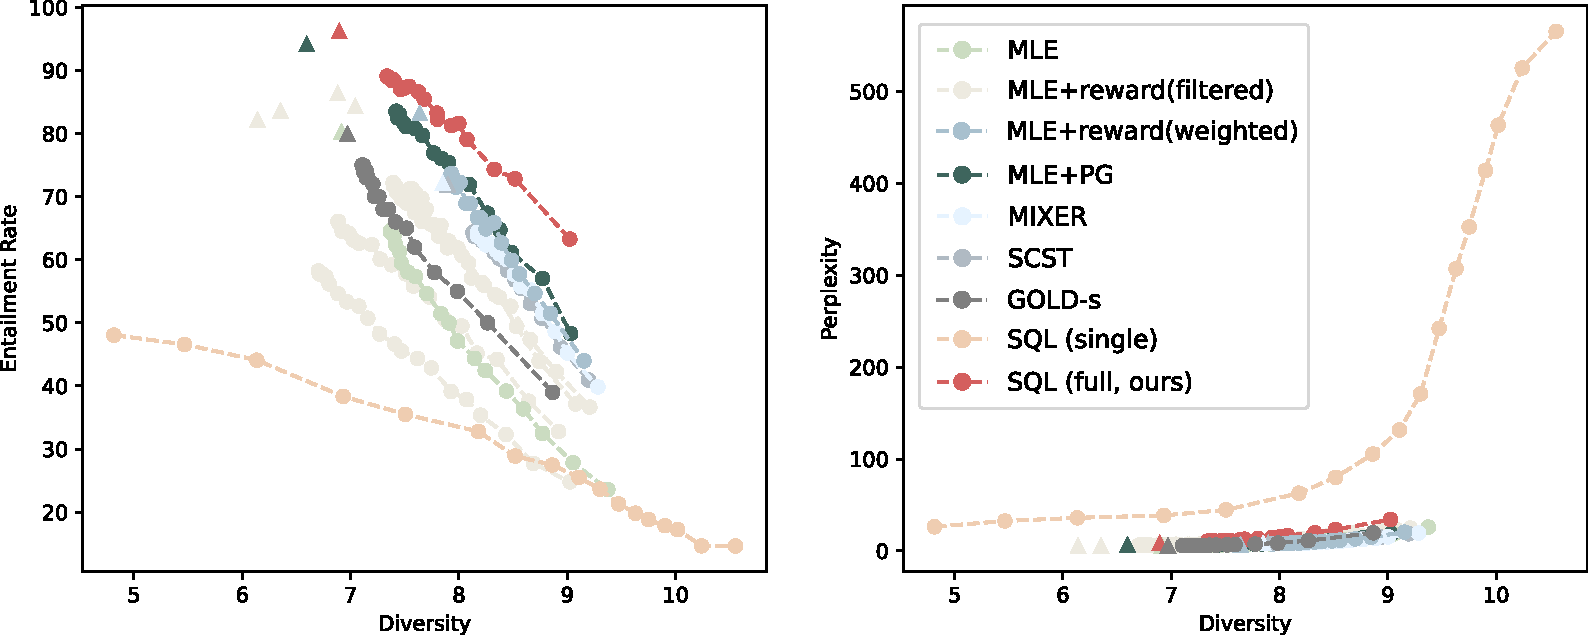
\includegraphics[width=0.86\linewidth]{figures/202101004-entailment-generation.all.pdf}
    \vspace{-4pt}
    \caption{Entailment generation performance plotted against diversity (average of $H_1$ and $H_2$).}
    \label{appendix-fig:entailment-generation}
    \vspace{-5pt}
\end{figure*}

\subsubsection{Learning from Noisy (Negative) Text}
\label{appendix-subsubsec:experiments-noisy-data}
Please see Table~\ref{table:entailment-generation} for beam search results, Figure~\ref{appendix-fig:entailment-generation} for additional results for \texttt{MLE+reward}, and Table~\ref{table:entailment-generation-examples-sql} for examples.


\subsubsection{\textit{Universal} Adversarial Attacks}
Please see Table~\ref{table:entailment-attack-examples} for examples.

\subsubsection{Prompt Generation for Controlling Pretrained Language Models}
\label{appendix-subsubsec:experiments-prompt-generation}
Please see Table~\ref{table:prompt-generation-full} for detailed results breakdown, and Table~\ref{table:prompt-examples-sql}-\ref{table:prompt-examples-pplm} for examples. Examples are in the format: \textcolor{red}{topic}: \textcolor{blue}{[prompt]} \textcolor{brown}{input sentence} generated text.

\subsubsection{Supervised Text Generation Tasks}
\label{appendix-subsec:standard-tasks}

Finally, we conduct experiment on standard generation tasks where clean supervised data is available. The study is to examine the capabilities of the proposed RL method to train a text generation model \emph{from scratch}, which has been considered as exceedingly challenging for previous RL algorithms.



\begin{table}
\centering
\small
\begin{tabular}{@{}l|llll@{}}
\toprule
\textbf{Model} & MLE & PG & MLE+PG & SQL (ours) \\
\midrule
\textbf{val} & $45.67$ & $0.00$ & $49.08$ & $47.04$ \\
\textbf{test} & $41.75$ & $0.00$ & $42.26$ & $41.70$ \\
\bottomrule
\end{tabular}
\vspace{-5pt}
\caption{BLEU results on the E2E val/test sets.}
\label{table:e2e-results}
\end{table}


\paragraph{Setup.}
We study on two tasks, E2E \citep{novikova2017e2e} and CommonGEN \citep{lin-etal-2020-commongen}, and use the respective datasets pre-processed by \citep{gehrmann2021gem} which allow sequence-to-sequence modeling with standard transformers.
We run four sets of methods:
the standard MLE training (\texttt{MLE}); PG training from scratch (\texttt{PG}); joint MLE and PG training, with MLE initialization (\texttt{MLE+PG}); and our SQL training from scratch with both off-policy and on-policy updates (\texttt{SQL}). We use the standard BLEU as reward.
We additionally investigate the training stability and sensitivity w.r.t hyperparameters, in particular the scale of reward. To this end, for \texttt{MLE+PG} and \texttt{SQL}, we vary the reward scale in $\{1, 10, 50, 100, 500, 1000\}$ and evaluate the respective performance under different scales.


\begin{figure*}
    \centering
    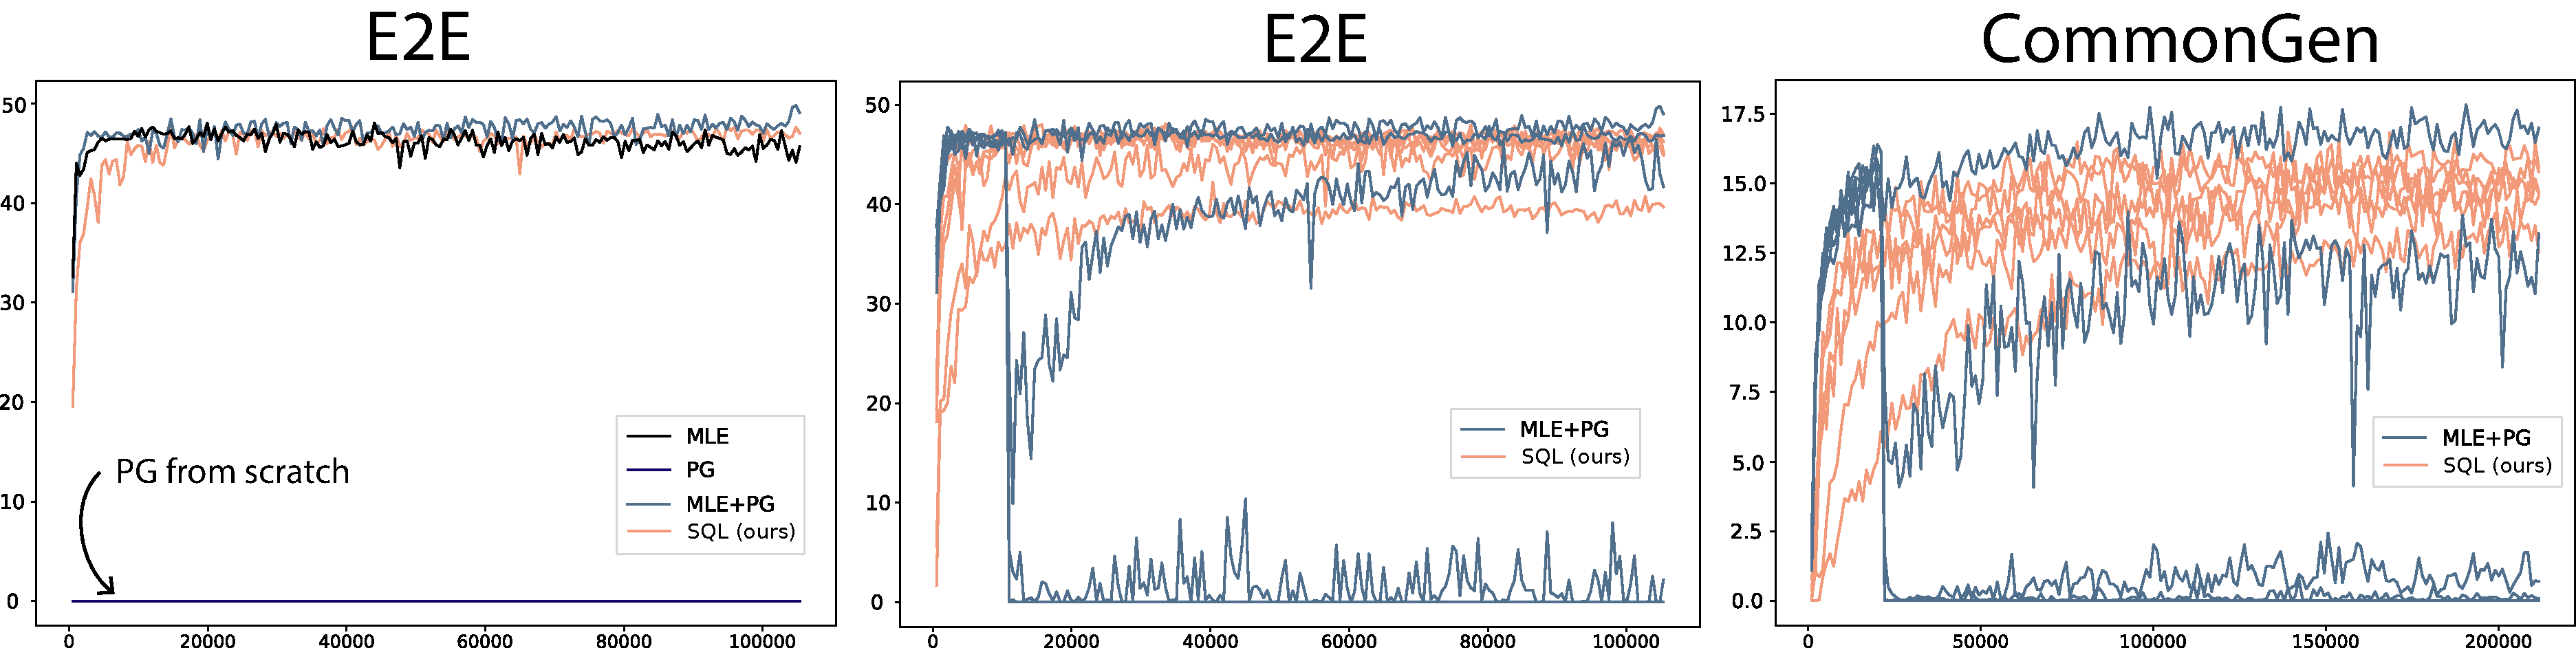
\includegraphics[width=0.99\linewidth]{figures/20210530.standard-tasks-small.pdf}
    \caption{Training curves on validation sets. {\bf Left:} Training curves on E2E with best hyperparameter configurations. {\bf Middle:} Training curves on E2E with varying reward scale. {\bf Right:} Training curves on CommonGen with varying reward scale.
    }
    \label{fig:supervised-text-generation-tasks}
\end{figure*}

\paragraph{Results.}
Table~\ref{table:e2e-results} shows the performance on E2E of different models whose hyperparameters are picked using the validation set. We can see the proposed \texttt{SQL} that trains models from scratch achieves competitive results with the common \texttt{MLE} and \texttt{MLE+PG}. In contrast, the \texttt{PG} algorithm alone without MLE fails the training. Figure~\ref{fig:supervised-text-generation-tasks} (left) shows the respective training curves (on the validation set), demonstrating that \texttt{SQL} converges in an efficient and stable way as \texttt{MLE}.

We further demonstrate the sensitive of \texttt{MLE+PG} and \texttt{SQL} w.r.t the reward scale as a key hyperparameter. Figure~\ref{fig:supervised-text-generation-tasks} (middle and right) shows the training curves of the two methods with varying reward scales. We can see \texttt{SQL} is significantly more robust as reward scale changes, while \texttt{MLE+PG} tends to collapse with improper reward scale configurations. 







\subsection{Setup Details}
\label{appendix-subsec:setup-details}

Our evaluation follows the GEM Benchmark~\citep{gehrmann2021gem} when applicable,\footnote{\url{https://github.com/GEM-benchmark/GEM-metrics}} and otherwise same with the reward function used in training. 
We use a transformer model~\citep{vaswani2017attention} based on Texar-Pytorch~\citep{hu2019texar} by default, with $64$ hidden dimension, $3$ blocks, and $4$ heads. 
For experiments that involve policy gradient training, we initialize the model with maximum likelihood training by default unless specified otherwise. We train soft $Q$-learning model from scratch with both off-policy (using data) and on-policy (using samples) by default except in \S\ref{subsec:noisy-data} and \S\ref{subsec:prompt-generation}, in which we find it beneficial to warm-up the model with just off-policy training. We apply similar tuning budgets to both soft $Q$-learning model, and policy-gradient (mostly the reward scale and top-$k$), based on performance on the validation dataset and sample qualities. Most of the experiments are conducted using Nvidia 1080 or 2080 series GPUs with around $12$GB memory. Most of the datasets are based in English.











\paragraph{Reward Functions}
We use the robust entailment classifier~\citep{nie2020adversarial} in \S\ref{subsec:noisy-data},\footnote{\url{https://huggingface.co/ynie/roberta-large-snli_mnli_fever_anli_R1_R2_R3-nli}. $355$M parameters.} one of the most used entailment classifiers on HuggingFaceHub in \S\ref{subsec:adversarial-attack},\footnote{\url{https://github.com/pytorch/fairseq/tree/master/examples/roberta}. This classifier is \textbf{ranked \#1} (as of May 20, 2021) based on \url{https://huggingface.co/models?search=nli}. $355$M parameters.} and a zero-shot classifier based on BART~\citep{lewis2020bart} to compute the topic score in \S\ref{subsec:prompt-generation}.\footnote{\url{https://huggingface.co/facebook/bart-large-mnli}. $407$M parameters.} To compute perplexities, we use a GPT-2 model ($124$M parameters)~\citep{radford2019language} fine-tuned on the corresponding datasets for computing perplexity in \S\ref{subsec:noisy-data} and~\ref{subsec:adversarial-attack}, and a distilled GPT-2 model in \S\ref{subsec:prompt-generation} without fine-tuning.\footnote{\url{https://huggingface.co/distilgpt2}. $82$M parameters.} We simply set reward weights to $1.0$, except in \S\ref{subsec:adversarial-attack}, where we changed the entailment weight to $0.5$, log-likelihood and repetition penalty weight to $5.0$. 




\subsubsection{Setup Details: \S\ref{subsec:noisy-data}}
\label{appendix-subsubsec:setup-noisy-data}
We study using the SNLI dataset~\citep{bowman2015large}, a dataset commonly used in training an entailment classifier. 
The original dataset contains \emph{(premise, hypothesis)} sentence pairs, where the hypothesis may or may not entail the premise. 
We sub-sampled $50,000$ training examples from the corpus such that the hypotheses have an average entailment probability of only $50\%$ in terms of the premises, and over $2/5$ examples have entailment probabilities less than $20\%$, which can be seen as negative (contradictive) examples. The resulting training set poses a significant challenge for the models to learn from the noises.


The RL algorithms (including PG and ours) permit us to plug in arbitrary reward functions to drive learning. Based on the goal of the task, we use the following intuitive rewards to ensure entailment accuracy and language quality: (1) a robust entailment classifier~\citep{nie2020adversarial} that measures the entailment score of a generation in terms of the input premise, (2) a GPT-2 language model~\citep{radford2019language} that measures the log-likelihood of the generation as an indicator of language quality, and (3) BLEU score w.r.t the input premises as another language quality reward that avoids trivial outputs. We sum together all rewards with weights $1.0$.



\begin{table}
\centering
\small
\begin{tabular}{@{}p{0.09\textwidth}|p{0.31\textwidth}lc@{}}
\toprule
Model & Generation                                                            & Rate \\
\midrule
MLE+PG    & it 's .                                                              & 90.48 \\
SQL (ours)  & the person saint-pierre-et-saint-paul is saint-pierre-et-saint-paul . & 97.40 \\
\bottomrule
\end{tabular}
\vspace{-5pt}
\caption{
Entailment attack samples and respective entailment rates across all test premises. For example, the adversarial sample by \texttt{SQL} is considered to entail 97.40\% test premises by the entailment classifier.
}
\label{table:entailment-attack-examples}
\end{table}

\subsubsection{Setup Details: \S\ref{subsec:adversarial-attack}}
\label{appendix-subsubsec:setup-adversarial-attack}
We study the task of attacking an entailment classifier. 
In particular, we aim to attack one of the most popular entailment classifiers on HuggingFaceHub.\footnote{\url{https://github.com/pytorch/fairseq/tree/master/examples/roberta}, which is ranked \#1 as of May 20, 2021 based on \url{https://huggingface.co/models?search=nli}.} 
The attack generation model generates adversarial text without conditioning on any inputs so that the generated attacks are universal to all premises.  
The generation model is trained with mostly the same setting as in \S\ref{subsec:noisy-data}, where the entailment classifier to be attacked is used as entailment score reward functions. Besides, we additionally include a token-level repetition penalty reward, which empirically benefits readability.
Finally, we use the MultiNLI dataset~\citep{williams2018broad} which includes more diverse examples than the SNLI used above. 

We compare our \texttt{SQL} with \texttt{MLE+PG}. We use all hypotheses in the MultiNLI dataset as the training data for the MLE training in \texttt{MLE+PG} and the off-policy updates for our \texttt{SQL}.
We do not compare with previous specialized adversarial text attack methods, because they either are not applicable to the universal attack setting \citep{morris2020textattack,jin2020bert,ebrahimi2017hotflip}, or were not designed to generate human-readable sentences \citep{wallace2019universal}. Besides, it is worth noting that the general RL algorithms have an additional advantage of doing \textit{black-box} attacks. That is, the algorithms only require the ability to query the entailment classifier for entailment probability, without need of knowing the internal structure of the classifier (e.g., for computing gradients) as in previous attack algorithms \citep{ebrahimi2017hotflip,wallace2019universal}.





For top-$p$ sampling results, we sample a hypothesis for each premise and measure the average attack rate across the dataset. This is because sampling multiple hypotheses, each for all premises, and measure performance are expensive. Since the hypotheses are sampled input-independently, this should be a good approximation.

\subsubsection{Setup Details: \S\ref{subsec:prompt-generation}}
\label{appendix-subsubsec:setup-prompt-generation}
Following \citep{dathathri2019plug}, we aim to control the generation to have one of 7 topics (e.g., ``science''); the generated prompt is prepended to one of 20 input sentences (Figure~\ref{fig:prompt-generation-flow}) for the pretrained LM to generate continuation sentences.
There is no direct supervision data available for training the prompt generator. We randomly create some noisy text as the training data for MLE baselines below and for off-policy updates for our algorithm. Specifically, the noisy text is created by sampling keywords and topics from the list used in \citep{Dathathri2020Plug} and a paraphrase generation model.

Figure~\ref{fig:prompt-generation-flow} shows the architecture of prompt-based controllable generation. We compare our \texttt{SQL} method with \texttt{MLE+PG} as before. At training time, for each generated prompt sample, the pretrained LM generates 2 continuation sentences for evaluating average reward. We use a \emph{zero-shot} classifier to evaluate the topic accuracy of the continuation sentences. That is, we do not assume access to classifiers pretrained on topic-specific sentences, because generating such topic-specific sentences is the goal of the task in the first place. We additionally use an LM to evaluate the log-likelihood of continuation sentences for measuring language quality. Since the prompt length could impact the generated sentences, we conducted experiments with maximum prompt length $5$, $10$, and $15$. As ablation study, we also evaluate the SQL algorithm with only off-policy updates (i.e., without on-policy exploration), denoted as \texttt{SQL(off)}, and compare it with vanilla \texttt{MLE} training. At test time, given a topic, the trained prompt generator produces one prompt using beam search decoding. For each generated prompt, the pretrained LM generates 100 sentences using top-$k$ decoding (with $k=50$) for evaluation. Finally, we also compare with two specialized controllable generation techniques based on pretrained LMs, namely \texttt{PPLM}~\citep{dathathri2019plug} and \texttt{GeDi}~\citep{krause2020gedi}, following similar procedures using their open-sourced code. We use a distilled GPT-2 model\footnote{\url{https://huggingface.co/distilgpt2}} as the pretrained LM to be controlled.

We use the paraphrase generation model based on~\citet{zhang2019pegasus}.\footnote{\url{https://huggingface.co/tuner007/pegasus_paraphrase}} During decoding, we include \texttt{no\_repeat\_ngram\_size}$=2$, which improves readability.\footnote{\url{https://huggingface.co/blog/how-to-generate}}




\subsection{The Soft $Q$-Learning Framework}
\subsubsection{Comparison with MLE Objective}
\label{comparison-with-mle-objective}
It is interesting to take a closer look at the above objective and compare with the common MLE training. 
Specifically, we notice the relations between the optimal $Q^*$, $V^*$, and $A^*$ functions: $A^*\left(\bm{s}_{t}, a_{t}\right) = Q^*(\s_t, a_t) - V^*(\s_t) = r_t + \gamma V^*(\s_{t+1}) -V^*\left(\bm{s}_{t}\right)$, where the first equation is the definition of $A^*$ (see Eq.\ref{eq:sql-state-value}) and the second equation is due to Eqs.\eqref{eq:q-and-next-v} and \eqref{eq:sql-state-value}. We thus can see the regression target in the above objective as an approximation to the advantage function: $\tilde{A}_{\bar{{\theta}}}\left(\bm{s}_{t}, a_{t}\right) := -V_{\bar{{\theta}}}\left(\bm{s}_{t}\right)+ \gamma V_{\bar{{\theta}}}\left(\bm{s}_{t+1}\right)+r_{t}$. Therefore, by optimizing the regression objective, $\log \pi_\theta(a_t|\s_t)$, which is the log probability of generating token $a_t$ given preceding tokens $\s_t$, is encouraged to match the approximate advantage value $\tilde{A}_{\bar{{\theta}}}\left(\bm{s}_{t}, a_{t}\right)$, no more and no less. This is different from the objective of MLE where the model is trained to (blindly) increase the probability of the observed token $a_t$ given $\s_t$ and decrease the probability of the rest.



\subsubsection{Vanilla Training with Temporal Consistency}
\label{appendix-subsubsec:vanilla-training-with-temporal-consistency}
Much like the Bellman temporal consistency in standard $Q$-learning, in SQL, the optimal action-value function follows the \emph{softmax} form of the temporal consistency~\citep{ziebart2008maximum,ziebart2010modeling,fox2016taming,nachum2017bridging}:
\begin{equation}
\small
    Q^{*}\left(\bm{s}_{t}, a_{t}\right) =r_{t} + \gamma \log \sum\nolimits_{a_{t+1}} \exp Q^*\left(\bm{s}_{t+1}, a_{t+1}\right) .
    \label{eq:q-and-next-v}
\end{equation}
We thus can derive a regression objective similar to the standard $Q$-learning (Eq.\ref{eq:q-regression}):
\begin{equation}
\small
\begin{aligned}
&\loss_{\text{SQL, vanilla}} (\bm{\theta}) \\
&= \mathbb{E}_{\pi'} \Bigg[ 0.5 \cdot \Bigg( r_t + \gamma \log \sum_{a_{t+1}} \exp Q_{\bar{{\theta}}}\left(\bm{s}_{t+1}, a_{t+1}\right) - Q_{{\theta}}\left(\bm{s}_{t}, a_{t}\right)\Bigg)^{2}\,\Bigg].
\label{eq:optimal-Q-2}
\end{aligned}
\end{equation}
Recall that $\pi'$ is an arbitrary behavior policy (e.g., data distribution), and $Q_{\bar{{\theta}}}$ is the target $Q$-network which is a slow copy of the $Q_\theta$ to be learned and is held fixed during the gradient updates. However, the above objective is inefficient due to exact the same reasons as in standard $Q$-learning discussed earlier, namely the unstable per-step bootstrapping-style training with sparse reward signals, plus the slow updates w.r.t only one token $a_t$ out of the large vocabulary (action space).


\begin{table*}
\centering
\small
\begin{tabular}{l|llllll}
\toprule
\textbf{Model} & \textbf{Entl. Prob $\uparrow$} & \textbf{Entl. Rate $\uparrow$} & \textbf{PPL  $\downarrow$} & \textbf{$H_1$ $\uparrow$} & \textbf{$H_2$ $\uparrow$} \\
\midrule
MLE    & $75.62$/$75.86$ & $79.75$/$80.23$ & $5.49$/$5.45$  & $5.46$/$5.42$ & $8.47$/$8.40$ \\
GOLD-s~\citep{pang2021text} & $74.55$/$76.03$ & $78.69$/$79.89$ & $5.55$/$5.50$  & $5.50$/$5.49$ & $8.48$/$8.45$ \\
MLE+PG & $90.16$/$89.73$ & $95.18$/$94.13$ & $6.38$/$6.31$ & $5.23$/$5.20$ & $8.02$/$7.99$ \\
SQL    & $91.94$/$91.55$ & $96.26$/$96.21$ & $8.41$/$8.42$ & $5.59$/$5.58$ & $8.20$/$8.21$ \\
SQL (single)$^\dagger$ & $89.90$/$89.92$ & $94.94$/$94.82$ & $214.42$/$214.42$ & $0.00$/$0.00$ & $0.00$/$0.00$ \\
\bottomrule
\end{tabular}
\caption{Beam search results on entailment generation, in the format \textbf{val/test}. $\uparrow$/$\downarrow$ indicates higher/lower is better. $^\dagger$\texttt{SQL (single)} achieves zero in $H_1$/$H_2$ as it generates a single token.
}
\label{table:entailment-generation}
\end{table*}






\begin{table*}
\centering
\small
\begin{tabular}{p{0.05\textwidth}l|p{0.06\textwidth}p{0.07\textwidth}p{0.09\textwidth}p{0.06\textwidth}p{0.07\textwidth}p{0.07\textwidth}p{0.07\textwidth}|>{\boldmath}l}
\toprule
\textbf{Length} & \textbf{Model} & \textbf{legal} & \textbf{politics} & \textbf{computers} & \textbf{space} & \textbf{religion} & \textbf{science} & \textbf{military} & \textbf{Average} \\
\midrule
\multicolumn{10}{c}{\textbf{Topic Scores}} \\
\midrule
/ & PPLM & $16.52$ & $25.09$ & $13.35$ & $26.23$ & $5.39$ & $38.87$ & $19.33$ & $20.68$ \\
/ & GeDi & $40.51$ & $83.40$ & $9.32$ & $70.90$ & $18.69$ & $12.46$ & $86.40$ & $45.96$ \\
5 & MLE       & $17.28$ & $13.44$ & $7.26$ & $42.27$ & $45.24$ & $39.31$ & $63.75$ & $32.65$ \\
5 & SQL (off) & $23.79$ & $61.11$ & $24.07$ & $7.91$ & $61.77$ & $64.67$ & $67.83$ & $44.45$ \\
5 & MLE+PG    & $29.45$ & $74.16$ & $72.49$ & $57.39$ & $65.62$ & $74.31$ & $76.86$ & $64.33$ \\
5 &  SQL      & $11.79$ & $70.57$ & $66.37$ & $58.80$ & $65.60$ & $69.24$ & $83.15$ & $60.79$ \\
10 & MLE+PG   & $17.72$ & $75.29$ & $71.01$ & $73.92$ & $58.29$ & $80.85$ & $80.84$ & $65.42$ \\
10 & SQL      & $29.62$ & $86.58$ & $75.72$ & $58.38$ & $71.29$ & $81.05$ & $91.40$ & $70.58$ \\
15 & MLE+PG   & $40.18$ & $81.47$ & $47.14$ & $82.64$ & $76.21$ & $84.82$ & $89.31$ & $71.68$ \\
15 & SQL      & $48.08$ & $77.94$ & $70.04$ & $87.43$ & $75.46$ & $85.94$ & $77.36$ & $74.61$ \\
\midrule
\multicolumn{10}{c}{\textbf{Perplexity}} \\
\midrule
/ & PPLM & $13.52$ & $12.81$ & $12.79$ & $13.56$ & $12.98$ & $12.43$ & $13.38$ & $13.07$ \\
/ & GeDi & $204.44$ & $80.01$ & $132.82$ & $116.94$ & $132.19$ & $90.00$ & $110.77$ & $123.88$ \\
5 & MLE       & $24.52$ & $25.05$ & $23.79$ & $26.26$ & $26.07$ & $25.63$ & $28.56$ & $25.70$ \\
5 & SQL (off) & $25.48$ & $22.70$ & $25.10$ & $26.64$ & $25.84$ & $27.45$ & $27.19$ & $25.77$ \\
5 & MLE+PG   & $24.42$ & $22.60$ & $27.74$ & $23.17$ & $25.38$ & $24.84$ & $30.50$ & $25.52$ \\
5 & SQL      & $25.31$ & $24.15$ & $26.40$ & $24.31$ & $27.02$ & $25.73$ & $28.67$ & $25.94$ \\
10 & MLE+PG   & $28.25$ & $23.49$ & $27.82$ & $26.88$ & $31.62$ & $25.31$ & $33.74$ & $28.16$ \\
10 & SQL      & $25.23$ & $25.37$ & $26.20$ & $26.97$ & $25.02$ & $27.11$ & $32.76$ & $26.95$ \\
15 & MLE+PG   & $28.38$ & $28.24$ & $28.16$ & $27.21$ & $26.43$ & $29.99$ & $32.54$ & $28.71$ \\
15 & SQL      & $35.16$ & $27.72$ & $29.70$ & $31.89$ & $24.04$ & $28.46$ & $26.74$ & $29.10$ \\
\bottomrule
\end{tabular}
\caption{Prompt generation results. Note that some of the numbers from GeDi are low because the topics are tokenized into two subword tokens, which the model was not trained with. 
}
\label{table:prompt-generation-full}
\end{table*}












\begin{table*}
\centering
\small
\begin{tabular}{p{0.97\textwidth}}
\toprule
\textcolor{red}{Input}: two men on bicycles competing in a race . \\
\textcolor{blue}{Generated}: two men are riding bikes . \\
\midrule
\textcolor{red}{Input}: families waiting in line at an amusement park for their turn to ride . \\
\textcolor{blue}{Generated}: families at a amusement park . \\
\midrule
\textcolor{red}{Input}: man in a black suit , white shirt and black bowtie playing an instrument with the rest of his symphony surrounding him . \\
\textcolor{blue}{Generated}: a man is playing music . \\
\midrule
\textcolor{red}{Input}: a white dog with long hair jumps to catch a red and green toy . \\
\textcolor{blue}{Generated}: a dog is jumping \\
\midrule
\textcolor{red}{Input}: a man in a black shirt is playing golf outside . \\
\textcolor{blue}{Generated}: a man is playing golf \\
\midrule
\textcolor{red}{Input}: a man wearing sunglasses is sitting on the steps outside , reading a magazine . \\
\textcolor{blue}{Generated}: a man is sitting outside . \\
\midrule
\textcolor{red}{Input}: a young child is jumping into the arms of a woman wearing a black swimming suit while in a pool . \\
\textcolor{blue}{Generated}: a child is jumping into a pool . \\
\midrule
\textcolor{red}{Input}: a carefully balanced male stands on one foot near a clean ocean beach area . \\
\textcolor{blue}{Generated}: a man is on the beach . \\
\midrule
\textcolor{red}{Input}: two young boys in swimming trunks are in the water looking at each other . \\
\textcolor{blue}{Generated}: two boys are in the water . \\
\midrule
\textcolor{red}{Input}: a woman riding a bicycle past a car and a group of people on a sidewalk . \\
\textcolor{blue}{Generated}: a woman rides a bicycle . \\
\midrule
\textcolor{red}{Input}: a female sings and plays into a microphone and a male in green striped shorts plays a hand drum \\
\textcolor{blue}{Generated}: a woman is playing music . \\
\midrule
\textcolor{red}{Input}: a little girl wearing a cardboard diner hat is finishing off some onion rings at a restaurant . \\
\textcolor{blue}{Generated}: a little girl is at a restaurant . \\
\midrule
\textcolor{red}{Input}: young woman celebrates getting a strike during a bowling game . \\
\textcolor{blue}{Generated}: a young woman is present \\
\midrule
\textcolor{red}{Input}: black greyhound dog racing down a track . \\
\textcolor{blue}{Generated}: a dog runs down a track . \\
\midrule
\textcolor{red}{Input}: several men on stage having a discussion . \\
\textcolor{blue}{Generated}: men are talking on stage . \\
\bottomrule
\end{tabular}
\vspace{5pt}
\caption{Entailment generation samples from SQL (beam search, validation dataset).}
\label{table:entailment-generation-examples-sql}
\end{table*}



\begin{table*}
\centering
\small
\begin{tabular}{p{0.95\textwidth}}
\toprule
\textcolor{red}{legal}: \textcolor{blue}{legal space religion and space} \textcolor{brown}{In summary}, a good understanding of these concepts is that by giving an explicit understanding to a person, they provide an avenue to be studied and studied. But the concept of one person being a space is also very confusing, and can be very difficult to obtain.\textbackslash n So, \\
\textcolor{red}{politics}: \textcolor{blue}{the primary referendum is} \textcolor{brown}{In summary}, the outcome will be a referendum on the EU membership for the first time of its kind for EU citizens, and the full extent of the benefits of a single market and a flexible single EU state." \\
\textcolor{red}{computers}: \textcolor{blue}{macintoshintoshintoshintosh} \textcolor{brown}{In summary}, it appears that the company and IBM products are currently in need of upgrading the computer. This can be seen in a detailed review of the Macintosh version of Windows Vista and XP. However, when looking at the changes made by the HP Macintosh hardware and software versions of \\
\textcolor{red}{space}: \textcolor{blue}{legal space science and space} \textcolor{brown}{In summary}:\textbackslash n\textbackslash n The purpose of this paper is to investigate and test the theory of space space and other objects. This project will support NASA.s efforts to demonstrate these theories, and to propose other relevant new theories.\textbackslash n This paper provides the following arguments for the \\
\textcolor{red}{religion}: \textcolor{blue}{space legal religion religion religion} \textcolor{brown}{In summary}, to the author the current discussion is the position of the Church and the community. While we acknowledge that we should not be commenting upon claims such as our recent cases or the other ones that contradict our view, we conclude it is appropriate to include these cases. Further \\
\textcolor{red}{science}: \textcolor{blue}{the chemical microscope is} \textcolor{brown}{In summary}, the most sophisticated of these experiments is a technique that gives no obvious, no apparent way of revealing that the material was obtained. In this study, we examine how the compounds in the samples in question make up the composition of the chemical and its properties. The chemical composition \\
\textcolor{red}{military}: \textcolor{blue}{arms defense battalion battalion cavalry} \textcolor{brown}{In summary}: 6th Panzer Field Division, Second Division.\textbackslash n\textbackslash n The main task of the battalion in the main counterinsurgency campaign was to counter the enemy in any counter-incursion. The main objective of this campaign is to eliminate enemy groups and the remnants of \\
\textcolor{red}{legal}: \textcolor{blue}{legal space religion and space} \textcolor{brown}{This essay discusses} the idea of space and time as a space, in both theoretical and conceptual terms, as not an individual time period or anything else. The emphasis is on time itself, rather than having a fixed central space. Space was the object of the first chapter, and \\
\textcolor{red}{politics}: \textcolor{blue}{the primary referendum is} \textcolor{brown}{This essay discusses} the nature of the EU referendum. The purpose of this essay is to shed light on the importance of a public referendum, on a question of whether the decision of an EU member states to remain in the European Union is constitutional and thus in accord with constitutional guarantees of sovereignty \\
\textcolor{red}{computers}: \textcolor{blue}{macintoshintoshintoshintosh} \textcolor{brown}{This essay discusses} hardware devices and software systems for Mac OS X, MacOS X and Linux. To view the latest version of Macintosh OS: Mac 8.7.x\textbackslash n\textbackslash n For more information or for information about Macintosh systems, visit Mac MacSystems.\textbackslash n More \\
\textcolor{red}{space}: \textcolor{blue}{legal space science and space} \textcolor{brown}{This essay discusses} science for teens, adults and teenagers.\textbackslash n\textbackslash n When the idea of studying space was first implemented as a method to test, the question was: What if a student has been "comfortable" with space without its body? What would their body like to be \\
\textcolor{red}{religion}: \textcolor{blue}{space legal religion religion religion} \textcolor{brown}{This essay discusses} an alternative religion that focuses on the role of a particular religion and views some form of religious ethics as the form when the law is applied to that particular religious community . This discussion is concerned with the status of faith for individuals or groups which may be members and members \\
\textcolor{red}{science}: \textcolor{blue}{the chemical microscope is} \textcolor{brown}{This essay discusses} the mechanisms of reaction with a focus on the molecular structure of nucleite and of enzymes within the cytoskeleton, thus making it easier to understand the process of metabolism and other elements of cellular life. In this essay, we use techniques such as the photochemical transfer \\
\textcolor{red}{military}: \textcolor{blue}{arms defense battalion battalion cavalry} \textcolor{brown}{This essay discusses} three main themes:\textbackslash n\textbackslash n 1) Lack of uniformed soldiers is an unacceptable and unconscionable strategy for the Army.\textbackslash n 2) Poor and inadequate training does not compensate the soldiers, and may deprive them of the necessary and competitive training from their instructors \\
\bottomrule
\end{tabular}
\caption{Prompt samples from SQL.}
\label{table:prompt-examples-sql}
\end{table*}









\begin{table*}
\centering
\small
\begin{tabular}{p{0.95\textwidth}}
\toprule
\textcolor{red}{legal}: \textcolor{blue}{there liable injunction} \textcolor{brown}{In summary}, the court decided that defendants had a right to petition the high court to intervene, and therefore granted the injunction. However, a Court of Appeal decision in the US District Court ruled with no effect on the petitioned by the plaintiffs, citing two reasons.\textbackslash n\textbackslash n The US \\
\textcolor{red}{politics}: \textcolor{blue}{the primary referendum was} \textcolor{brown}{In summary}, the majority of Russians would support the idea of banning all human rights, and that would be a major part of the government’s effort to build a new liberal economy, which President Vladimir Putin says would boost Russian tourism.\textbackslash n\textbackslash n The results were published in the \\
\textcolor{red}{computers}: \textcolor{blue}{the macintoshintosh} \textcolor{brown}{In summary}, the kernel has the best quality of life, and kernel security is at the heart of any OS development. The first time Linux released was when i386 released the Macintosh version, which had a rather low standard. Other issues like the introduction of the OS6 operating system \\
\textcolor{red}{space}: \textcolor{blue}{comet asteroid spaceship} \textcolor{brown}{In summary}, this asteroid asteroid ship is about to make its maiden flight to explore deep-space.\textbackslash n\textbackslash n "The asteroid craft was a very early attempt at the discovery of a new home for the world's first black hole," NASA said in a news release. "Today we \\
\textcolor{red}{religion}: \textcolor{blue}{faith faith faith salvation} \textcolor{brown}{In summary}, Christian beliefs are not a new way to use the time spent thinking about God's world as a source for faith. Faith is an effort to think of the world without fear that it might become a dangerous place for the human family. Because it represents the very essence that \\
\textcolor{red}{science}: \textcolor{blue}{climate research chemistry} \textcolor{brown}{In summary} of the study, this review aims to determine how in a single study where the same number of data was analysed, a new methodology is needed to better understand who produced a different graph than the one suggested. The paper will be published in issue \#5, Issue \#18. \\
\textcolor{red}{military}: \textcolor{blue}{the cavalry battalion a} \textcolor{brown}{In summary}, the army are a unit of the same type and in all, so there is no need to declare one. The unit does not constitute a cavalry unit or for use on troops.\textbackslash n\textbackslash n The army is not under the command of a brigade from the front. For \\
\textcolor{red}{legal}: \textcolor{blue}{there liable injunction} \textcolor{brown}{This essay discusses} the potential legal consequences of a stay in the United States for an indefinite period of time if the government continues to delay the process of de-instituting it. To apply such a request, all applicable laws shall apply either the same terms as the existing statutes. In \\
\textcolor{red}{politics}: \textcolor{blue}{the primary referendum was} \textcolor{brown}{This essay discusses} the electoral strategy against a candidate for governor of the Commonwealth.\textbackslash n\textbackslash n The survey of British voters in this survey provides an overview of what the candidates for the United Kingdom will be seeking in the next Parliament. In the general election a few seats will lead up to a \\
\textcolor{red}{computers}: \textcolor{blue}{the macintoshintosh} \textcolor{brown}{This essay discusses} the various problems of the Macintosh, the first two-year running environment. An early version of this paper was originally published in 1982. The MacSX was not designed and managed by Kia.\textbackslash n\textbackslash n Macintosh\textbackslash n The mac has been a family invention \\
\textcolor{red}{space}: \textcolor{blue}{comet asteroid spaceship} \textcolor{brown}{This essay discusses} a topic: the impact of two of the Earth's two-thirds comet-sized moon Charon on Earth, and why asteroids are so close to the sun; why people are looking for ways to find a way to keep Earth-shaped asteroids out of orbit. \\
\textcolor{red}{religion}: \textcolor{blue}{faith faith faith salvation} \textcolor{brown}{This essay discusses} the impact religion has on the American experience and in American culture. Since the beginning of my career I have found that faith and belief have often been linked to economic growth, social development and education. I believe that all people need to know that there is no reason for \\
\textcolor{red}{science}: \textcolor{blue}{climate research chemistry} \textcolor{brown}{This essay discusses} the role of molecular information and its interaction with the general organism and human health.\textbackslash n\textbackslash n "The idea of biological information is not really a new concept. We used genetic information as a medium to define, identify, and store information about biology and biology," explains Dr. \\
\textcolor{red}{military}: \textcolor{blue}{the cavalry battalion a} \textcolor{brown}{This essay discusses} the potential for the development of a small infantry brigade as an infantry regiment. It is also a contribution to the larger cavalry corps as it would require a larger brigade for battle. For more information see the original article on this page. \\
\bottomrule
\end{tabular}
\caption{Prompt samples from MLE+PG.}
\label{table:prompt-examples-pg}
\end{table*}




\begin{table*}
\centering
\small
\begin{tabular}{p{0.95\textwidth}}
\toprule
\textcolor{red}{legal}: \textcolor{brown}{In summary} Currently: In 1966 the Act was amended into state of law through amendments.\textbackslash n\textbackslash n\textbackslash n Defent No. 1 etc 695 [The character in question for judicial decision purposes; participation t concerned you; "but not acceptance.")\textbackslash n\textbackslash n Generally held: Just \\
\textcolor{red}{politics}: \textcolor{brown}{In summary} Senate candidates, senator (Republican); senator (Democrat); and opinion-former (2002-08). - 2012 Senate results are based on the federal Election Commission's October 2016 Current Opinion Polling Reports. Key figures : Open Gallup poll Most Americans view the \\
\textcolor{red}{computers}: \textcolor{brown}{In summary}: 12-16 add-on chips. Trace out the type predefined ORDER parameters, and write to /dev/tty with them.\textbackslash n\textbackslash n\textbackslash n\textbackslash n\textbackslash n\textbackslash n\textbackslash n\textbackslash n\textbackslash n Roundset sizes with mm(831x810 x870 x81f); \\
\textcolor{red}{space}: \textcolor{brown}{In summary} Space Station - Farm Station (1985 by Mike Lazarra) Here is an article developed by Maregnus Spirit Experimentator on WinViotrv - An exploration benefit for compute-enriched array data densities (UPERS).This thesis home \\
\textcolor{red}{religion}: \textcolor{brown}{In summary} nice things about Android 6.1 Jelly Bean!\textbackslash n Searching for OP lag fixes one of my cllcs or some other improvements that's fixing a bug due to this nerf! (model causing Huge Frame Decay!) It also fixed an upper turret hook \\
\textcolor{red}{science}: \textcolor{brown}{In summary} Computer Age Experience Overview\textbackslash n\textbackslash n\textbackslash n\textbackslash n Networking skills are the most developed skill set for Internetthumb members at universities at this time. In computer science, we are introducing various gatekeepers to intellectual property ownership and cyberware acquisitions, entry program makers post a \\
\textcolor{red}{military}: \textcolor{brown}{In summary} Army Sgt. Harold Tolbard (5/16/2018) Lt. Gen. Michael Bachaes 1 Dickie Powell 2 Lt. Zachary Bram 9 *Gen. Robert Eisen: Warfighter – Soldier + Genoured\textbackslash n\textbackslash n\textbackslash n – Senior Bush Doctrine \\
\textcolor{red}{legal}: \textcolor{brown}{This essay discusses} Illinois cases on issues such as drug trafficking and drug Social Security. \\
\textcolor{red}{politics}: \textcolor{brown}{This essay discusses} federal ethics as the key area on which current and past state and local governments have been operating. \\
\textcolor{red}{computers}: \textcolor{brown}{This essay discusses} the very development of alternative technology for young people. \\
\textcolor{red}{space}: \textcolor{brown}{This essay discusses} NASA's StarHubble satellite mission development. Transcript here. \\
\textcolor{red}{religion}: \textcolor{brown}{This essay discusses} various aspects of the relays of mediocality and Hammazanna. \\
\textcolor{red}{science}: \textcolor{brown}{This essay discusses} Linux desktop computing, and IRI video-game applications.\textbackslash n\textbackslash n The zooming in — even after the GNOME 3 transition came to an end, is all about figuring out how you have run a software operating system so vital that any hacker can mine it \\
\textcolor{red}{military}: \textcolor{brown}{This essay discusses} military courage that included in the combat operations in Iraq and Afghanistan. \\
\bottomrule
\end{tabular}
\caption{Prompt samples from GeDi.}
\label{table:prompt-examples-gedi}
\end{table*}






\begin{table*}
\centering
\small
\begin{tabular}{p{0.95\textwidth}}
\toprule
\textcolor{red}{legal}: \textcolor{brown}{In summary} we have published in the journal Nature Neuroscience: A systematic review of human brain tissue has found no evidence for any association between the presence of the presence of a particular form of human neuropathy in the brain, a condition that is not normally associated with cognitive impairment. We found that \\
\textcolor{red}{politics}: \textcolor{brown}{In summary} we have a list of 10 of the best and most common types of drugs for people with HIV. This is a very short list of recommendations from a national and international community.\textbackslash n\textbackslash n\textbackslash n\textbackslash n This article has been updated to make the official state of the EU state of \\
\textcolor{red}{computers}: \textcolor{brown}{In summary}, we believe that the current system has no way of doing anything about it.\textbackslash n\textbackslash n\textbackslash n\textbackslash n The following steps are taken to get the system working.\textbackslash n\textbackslash n 1. Install a new operating system with a Linux Mint operating system\textbackslash n 2. Start a new Linux Mint operating \\
\textcolor{red}{space}: \textcolor{brown}{In summary} we have some important news from the moment of the year and some important information about these two major planets. This new discovery is the first to confirm this important planet has an active life in its home planet, a planet with a mass of about 5.8 billion tons. It \\
\textcolor{red}{religion}: \textcolor{brown}{In summary}, we believe that the current administration has no way of doing anything about the Benghazi attacks. This is a very interesting story, and I think it has been a very nice surprise. This is a very nice and well thought out piece that is a must for the \\
\textcolor{red}{science}: \textcolor{brown}{In summary} we use this approach to evaluate if the number of data points (in the dataset) that are relevant for each data set is the same (in this case, the data are not in one data set). In this approach we can test the data points in a different way. \\
\textcolor{red}{military}: \textcolor{brown}{In summary} we have some important news from the moment of the year and some important information from the moment of the year.\textbackslash n\textbackslash n\textbackslash n\textbackslash n\textbackslash n We've also added an additional update for our new feature, which includes:\textbackslash n • Improved access and access in all of the main \\
\textcolor{red}{legal}: \textcolor{brown}{This essay discusses} how you can build a community of dedicated people. If you're a member of a community of people who want to contribute to the environment, you'll also be helping them build communities in order to support the local economy, and the future of the city. The latest report \\
\textcolor{red}{politics}: \textcolor{brown}{This essay discusses} how we can build on previous research findings about the role religion plays in human development in human development. This is a very interesting and highly entertaining story. What is an "independent" political party in the United States, the U.S. political party, and the United \\
\textcolor{red}{computers}: \textcolor{brown}{This essay discusses} how you can build a new browser to view and share your favorite web sites.\textbackslash n\textbackslash n\textbackslash n A browser that is open source can also be built from a web browser, which can be a browser that does not allow browser extensions (e.g. Firefox, Chrome, Opera \\
\textcolor{red}{space}: \textcolor{brown}{This essay discusses} how you can build a life with a healthy diet and how you can use it when you're ready to move forward. It's a very simple approach to building a life with a healthy diet and what it means to be healthy and healthy for the \\
\textcolor{red}{religion}: \textcolor{brown}{This essay discusses} how you can build a new game without having to play the original game, and how you can make a new title that is completely different to the original. It has been around since 2007, when the first game, The Elder Scrolls IV: Oblivion, was released in the PlayStation \\
\textcolor{red}{science}: \textcolor{brown}{This essay discusses} how we can build on previous research findings about the role of obesity in human metabolism and how we can improve our health.\textbackslash n\textbackslash n\textbackslash n\textbackslash n In this essay, we explore why eating a whole whole diet does not help prevent obesity (1). We find that a whole food diet \\
\textcolor{red}{military}: \textcolor{brown}{This essay discusses} how you can build a community with the help of friends and family.\textbackslash n\textbackslash n\textbackslash n\textbackslash n\textbackslash n "The people around me are the ones who need help. They are the ones who need help. They are the ones who are not alone."\textbackslash n - Michael\textbackslash n "It's \\
\bottomrule
\end{tabular}
\caption{Prompt samples from PPLM.}
\label{table:prompt-examples-pplm}
\end{table*}